\chapter{Background}

In this chapter I am going to introduce the reader to the concepts that are necessary to understand the research presented in this thesis. The chapter is divided into three sections. The first section provides an overview of Variational Autoencoders (VAEs) and their applications. The second section introduces Vector Quantized VAEs (VQ-VAEs). The third section introduces the concept of semi-conditioned VAEs. The chapter is concluded with a section that introduces the concept of multitask learning. 

\section{VAEs}

Variational Autoencoders (VAEs), first introduced in 2013 by Kingma and Welling\cite{kingma2013autoencoding}, have become a prominent class of generative models in the field of machine learning.  At their core, VAEs consist of an encoder network with parameters $\phi$ that maps data points $x$ into a latent space $z$ and a decoder network with parameters $\theta$ that generates data $\hat{x}$ from latent representations\cite{Kingma_2019}. 

The key innovation that makes VAEs work is the introduction of a probabilistic interpretation of the latent space. More specifically, VAEs assume that the latent space $z$ is a random variable that follows a certain prior distribution $p(z)$, which is typically a Gaussian distribution and that the mapping from the latent space to the data space is also probabilistic\cite{kingma2013autoencoding}.

The optimization target for VAEs is the evidence lower bound (ELBO), which is
 \[ L_{\theta, \phi}(x) = \mathbb{E}_{q_{\phi}(z|x)} [\log p_{\theta}(x, z) - \log q_{\phi}(z|x)], \]
where $q_{\phi}(z|x)$ is the encoder distribution, $p_{\theta}(x, z)$ is the decoder distribution. 

The ELBO can be also written as a sum of two terms,
 \[ L_{\theta, \phi}(x) = - D_{KL}(q_{\phi}(z|x) || p(z)) + \mathbb{E}_{q_{\phi}(z|x)} [\log p_{\theta}(x|z)], \]
 where $D_{KL}(q_{\phi}(z|x) || p(z))$ is the Kullback-Leibler divergence between the encoder distribution $q_{\phi}(z|x)$ and the prior distribution $p(z)$ and $\mathbb{E}_{q_{\phi}(z|x)} [\log p_{\theta}(x|z)]$ is the reconstruction term. The Kullback-Leibler divergence term encourages the encoder distribution to be close to the prior distribution, while the reconstruction term encourages the reconstruction to be as accurate as possible\cite{Kingma_2019}.


Taking random samples from from $q_{\phi}(z|x)$, Monte Carlo estimate of ELBO can be written of this as
\[ L_{\theta, \phi}(x) = - D_{KL}(q_{\phi}(z|x) || p(z)) + \frac{1}{L} \sum_{l=1}^{L} \log p_{\theta}(x|z^{(l)}) ,\]
where $z^{(l)} \sim q_{\phi}(z|x)$ and $L$ is the number of samples and first term is the regularization term and the second term is the reconstruction term\cite{Kingma_2019}. 

The regularization term is the Kullback-Leibler divergence between the encoder distribution and the prior distribution. The regularization term encourages the encoder distribution to be close to the prior distribution. The reconstruction term is the reconstruction error of the decoder. The reconstruction term encourages the decoder to reconstruct the input data as accurately as possible.

The individual datapoint ELBO and it's gradient in general is intractable to compute. However, unbiased estimates of the ELBO and its gradients can be obtained using the reparametrization trick, which is described in the next section\cite{Kingma_2019}.


\subsection{Reparametrization Trick}

The Reparametrization trick also  is a crucial component of VAEs. It is used to make the ELBO differentiable with respect to the parameters of the encoder $\phi$ and decoder $\theta$ through a change of variables.\cite{Kingma_2019}

\subsubsection{Change of variables}

The notion is based on the fact that it is possible to express the random variable $z \sim q_{\phi}(z|x)$ as a differentiable function of a random variable $\epsilon$ and the parameters $\phi$ such that $z = g_{\phi}(\epsilon, x)$, where epsilon is a random variable that is independent of $\phi$ and $x$ and $\epsilon \sim p(\epsilon)$. Given this change of variables, the expection with respect to $q_{\phi}(z|x)$ can be rewritten as an expectation with respect to $p(\epsilon)$
\[ E_{q_{\phi}(z|x)}[f(z)] = E_{p(\epsilon)}[f(g_{\phi}(\epsilon, x))], \]
where $f$ is an arbitrary function.\cite{Kingma_2019}
As a result, the gradients the expectation and gradient operators become cummutive, and there can be formed a Monte Carlo estimate of the gradients
\[ \nabla_{\phi} E_{q_{\phi}(z|x)}[f(z)] = \nabla_{\phi} E_{p(\epsilon)}[ f(g_{\phi}(\epsilon, x))] \]
\[ = E_{p(\epsilon)}[\nabla_{\phi} f(g_{\phi}(\epsilon, x))] \]
\[  \simeq \frac{1}{L} \sum_{l=1}^{L} \nabla_{\phi} f(g_{\phi}(\epsilon^{(l)}, x)) \]
where $\epsilon^{(l)} \sim p(\epsilon)$ and $L$ is the number of samples.
This is the reparametrization trick, which is further explained and illustrated in the figure \ref{reparametrization}.

\begin{figure}
    \centering
    \begin{tikzpicture}[
    roundnode/.style={circle, draw=red!60, fill=red!5, very thick, minimum size=7mm},
    squarednode/.style={rectangle, draw=gray!60, fill=gray!5, very thick, minimum size=5mm},
    redarrow/.style={->, red, >=stealth, thick},
    redtext/.style={red}
    ]

    % Two boxes with widht of full text
    \draw (0,0) rectangle (6, 6);
    \draw (7,0) rectangle (13, 6);
    % Headlines
    \node[align=center] at (3,5.5) {Original Form};
    \node[align=center] at (10,5.5) {Reparametrized Form};

    % --- First box ---
    %Nodes
    \node[squarednode]      (function)      at(3, 4.5)                    {$f$};
    \node[roundnode]        (z)             [below= of function]          {$z$};
    \node[squarednode]      (x)             [below= of z]                 {$x$};
    \node[squarednode]      (phi)         [left= of x]        {$\phi$};
    %Lines
    \draw [->] (z) -- (function);
    \draw [->] (x) -- (z);
    \draw [->] (phi) -- (z);

    % --- Second box ---
    %Nodes
    \node[squarednode]      (function2)      at(10, 4.5)                    {$f$};
    \node[squarednode]        (z2)             [below= of function2]          {$z$};
    \node[squarednode]      (x2)             [below= of z2]                 {$x$};
    \node[squarednode]      (phi2)         [left= of x2]        {$\phi$};
    \node[roundnode]        (epsilon)        [right= of x2]        {$\epsilon$};
    %Lines
    \draw [->] (z2) -- (function2);
    \draw [->] (x2) -- (z2);
    \draw [->] (phi2) -- (z2);
    \draw [->] (epsilon) -- (z2);

    % draw back propagation with red line draw to the left
    \draw [redarrow] (9.5, 4.5) -- (9.5, 3.3);
    \node [redtext, above left= -0.3 and 0.3 of z2] { $\nabla_{z} f$};
    \draw [redarrow] (9.5, 3) -- (8.5, 2);
    \node [redtext, above left= -0.1 and -0.1 of phi2] { $\nabla_{\phi} f$};
    % One box below to show the meaning of nodes and lines
    \draw (0,-3) rectangle (13, -0.5);
    %show the meaning of nodes 
    \node[squarednode]    (square_explanation_node)    at(1, -1)    {};
    \node [right= 0.5 of square_explanation_node] {: Deterministic node};
    \node[roundnode]    (round_explanation_node)    at(1, -2)    {};
    \node [right= 0.5 of round_explanation_node] {: Random node} ;
    %\draw (5.5, -2)    node    {: Random node};
    %show the meaning of lines( with name of the line)
    \draw [->] (7, -1) -- (8, -1) node [right = 0.5,] { : Calculation of f};
    \draw [redarrow] (7, -2) -- (8, -2) node [right = 0.5,] { : Differentiation of f};
\end{tikzpicture}
    \caption[The illustration diagram of the reparametrization trick]%
    {The illustration diagram of the reparametrization trick. The input of a function $f$ is $x$. The parameters $\theta$ affect the objective of the function $f$ through a random variable $z$. In the original form we can not compute the gradients $\nabla_{\phi} f$, because a direct backpropagation is not possible through a random variable. In the reparameterized form, the randomness is seperated from the parameters $\phi$, which enables the gradients to be computed. This is done by reparameterizing the random variable $z$ as a deterministic function and differentiable function  of $\phi$, $x$ and a new random variable $\epsilon$.\cite{Kingma_2019}}

    \hspace*{15pt}\hbox{\scriptsize Credit: Adapted from Kingma and Welling\cite{Kingma_2019}  }\label{reparametrization}

\end{figure}

\subsubsection{Gradients of the ELBO}

When applying the reparametrization trick to the ELBO it becomes differentiable with respect to both $\phi$ and $\theta$ and it is possible to form a Monte Carlo estimate of the gradients
\[ \nabla_{\phi, \theta} L_{\theta, \phi}(x) = \nabla_{\phi, \theta} E_{q_{\phi}(z|x)} [\log p_{\theta}(x, z) - \log q_{\phi}(z|x)] \]
\[ = E_{p(\epsilon)}[\nabla_{\phi, \theta} [\log p_{\theta}(x, g_{\phi}(\epsilon, x)) - \log q_{\phi}(g_{\phi}(\epsilon, x)|x)]] \]
\[  \simeq \frac{1}{L} \sum_{l=1}^{L} \nabla_{\phi, \theta} [\log p_{\theta}(x, g_{\phi}(\epsilon^{(l)}, x)) - \log q_{\phi}(g_{\phi}(\epsilon^{(l)}, x)|x)] \]
where $\epsilon^{(l)} \sim p(\epsilon)$ and $L$ is the number of samples.

This is the key to training VAEs using stochastic gradient descent. The resulting Monte Carlo gradient estimate is used to update the parameters of the encoder and decoder networks.\cite{Kingma_2019}


\subsection{Gaussian VAEs}

Altough Gaussian VAEs are just a special case of VAEs, they are the most common type of VAEs. Gaussian VAEs assume that the prior distribution $p(z)$ is a centered Gaussian distribution $ p(z) = \mathcal{N}(0, I)$. They also assume that the decoder distribution $p_{\theta}(x|z)$ is a Gaussian distribution whose distribution parameters are computed from z with by the decoder network. The decoder distribution is given by
\[ p_{\theta}(x|z) = \mathcal{N}(f_{\theta}(z), I) \]
where $f_{\theta}(z)$ is the mean and $\sigma_{\theta}(z)$ is the standard deviation of the Gaussian distribution. Whilst there is a lot of freedom in the form $q_{\phi}(z|x)$ can take, Gaussian VAEs assume that $q_{\phi}(z|x)$ is also a Gaussian distribution with an approximately diagonal covariance matrix: 
\[ q_{\phi}(z|x) = \mathcal{N}(\mu_{\phi}(x), \sigma_{\phi}(x)) \]
where $\mu_{\phi}(x)$ and $\sigma_{\phi}(x)$ are the mean and standard deviation of the Gaussian distribution, which are computed by the encoder network.

To sample $z$ from $q_{\phi}(z|x)$, we can use the reparametrization trick described in the previous section
\[ z = \mu_{\phi}(x) + \sigma_{\phi}(x) \odot \epsilon, \] 
where $\epsilon \sim \mathcal{N}(0, I)$ is a random variable sampled from a standard Gaussian distribution and $\odot$ denotes element-wise multiplication.

When applying these assumptions to the ELBO, we get the following expression: \[ L_{\theta, \phi}(x) = - D_{KL}(q_{\phi}(z|x) || p(z)) + \frac{1}{L} \sum_{l=1}^{L} \log p_{\theta}(x|z^{(l)}) \]
\[ = - D_{KL}(\mathcal{N}(\mu_{\phi}(x), \sigma_{\phi}(x)) || \mathcal{N}(0, I)) + \frac{1}{L} \sum_{l=1}^{L} \log \mathcal{N}(x|f_{\theta}(z^{(l)}), I) \]
where $f_{\theta}(z^{(l)}) = f_{\theta}(\mu_{\phi}(x) + \sigma_{\phi}(x) \odot \epsilon^{(l)})$ and $\epsilon^{(l)} \sim \mathcal{N}(0, I)$.

However, the loss function to be \textbf{minimized} for VAE's usually used in practise is quite different from the ELBO negative. 
The function that is used in practice consists of: Mean Squared Error (MSE) reconstruction loss, KL divergence regularization loss and a constant $\beta$ that controls the importance of the regularization term
\[ L = \frac{1}{D} \sum_{i=1}^{D} ||x_i - \hat{x} ||^2 + \beta  \frac{1}{2} \biggl( -\log \sigma^2_\phi(x) - 1 + \mu^2_\phi(x) + \sigma^2_\phi(x) \biggr), \]
where $\hat{x} = f_{\theta}(\mu_{\phi}(x_i) + \sigma_{\phi}(x_i) \odot \epsilon^{(i)})$ and $\epsilon^{(i)} \sim \mathcal{N}(0, I)$, $D$ is the dimension of the input data. The second term in the function is derived from simplifing the KL divergence term in the ELBO, which is shown in the equation~\ref{eqKL}. The first term in the function is the MSE reconstruction loss because maximizing the Gaussian likelihood is approximately equivalent to minimizing the MSE reconstruction loss. This is shown in the equation~\ref{eqMSE}.
\begin{equation} \label{eqKL}
    \begin{split}
        D_{KL}(q_\phi(z|x) \| p_\theta(z)) &= \int q_\phi(z|x) \biggl[\ \log q_\phi(z|x) - \log p_\theta(z) \ \biggr] dz \\
        &= \int q_\phi(z|x) \biggl[\ -\frac{1}{2} \log (2\pi\sigma^2_\phi(x)) - \frac{(z - \mu_\phi(x))^2}{2\sigma^2_\phi(x)} \\
        &\qquad\qquad\qquad - \left( -\frac{1}{2} \log 2\pi - \frac{z^2}{2} \right) \ \biggr] \\
        &= \frac{1}{2} \int q_\phi(z|x) \biggl[ -\log \sigma^2_\phi(x) - \frac{(z - \mu_\phi(x))^2}{\sigma^2_\phi(x)} + z^2 \biggr] \\
        &= \frac{1}{2} \biggl( -\log \sigma^2_\phi(x) - 1 + \mu^2_\phi(x) + \sigma^2_\phi(x) \biggr)
    \end{split}
\end{equation}
\begin{equation} \label{eqMSE}
    \begin{split}
        \argmax_{\theta} \log \mathcal{N}(x|f_{\theta}(z), I) & = \argmax_{\theta} \log \biggl[\frac{1}{\sigma \sqrt{2\pi}} \exp \biggl( -\frac{1}{2 \sigma^2} (x - f_{\theta}(z))^2 \biggr)\biggr] \\
        & = \argmax_{\theta} \biggl[ \log \frac{1}{\sigma \sqrt{2\pi}} - \frac{1}{2 \sigma^2} (x - f_{\theta}(z))^2 \biggl]\\
        & = \argmin_{\theta} \frac{1}{2} (x - f_{\theta}(z))^2
    \end{split}
\end{equation}

In the figure belowe~\ref{VAEFigure} there is a visualization of the architecture of Gaussian VAEs.

\begin{figure}[H]
    \centering 
    \tikzset{every picture/.style={line width=0.75pt}} %set default line width to 0.75pt        

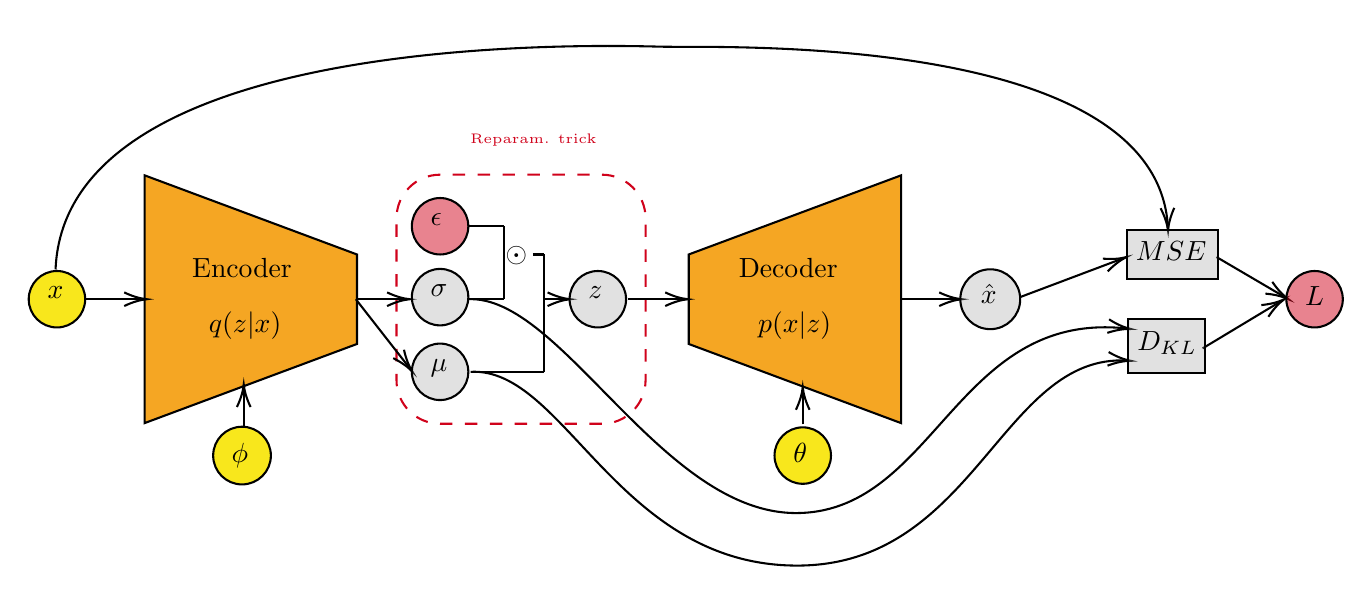
\begin{tikzpicture}[x=0.75pt,y=0.75pt,yscale=-1,xscale=1]
%uncomment if require: \path (0,300); %set diagram left start at 0, and has height of 300

%Shape: Trapezoid [id:dp7823603828525814] 
\draw  [fill={rgb, 255:red, 245; green, 166; blue, 35 }  ,fill opacity=1 ] (93.26,100.32) -- (195.56,138.44) -- (195.56,181.56) -- (93.26,219.68) -- cycle ;
%Flowchart: Alternative Process [id:dp7916519671015572] 
\draw  [color={rgb, 255:red, 208; green, 2; blue, 27 }  ,draw opacity=1 ][dash pattern={on 4.5pt off 4.5pt}] (313.6,100) .. controls (325.2,100) and (334.6,109.4) .. (334.6,121) -- (334.6,199) .. controls (334.6,210.6) and (325.2,220) .. (313.6,220) -- (235.6,220) .. controls (224,220) and (214.6,210.6) .. (214.6,199) -- (214.6,121) .. controls (214.6,109.4) and (224,100) .. (235.6,100) -- cycle ;
%Shape: Trapezoid [id:dp7878502215303758] 
\draw  [fill={rgb, 255:red, 245; green, 166; blue, 35 }  ,fill opacity=1 ] (457.69,219.68) -- (355.39,181.56) -- (355.39,138.44) -- (457.69,100.32) -- cycle ;
%Straight Lines [id:da7022493612643106] 
\draw    (65,160) -- (92.33,160) ;
\draw [shift={(94.33,160)}, rotate = 180] [color={rgb, 255:red, 0; green, 0; blue, 0 }  ][line width=0.75]    (10.93,-3.29) .. controls (6.95,-1.4) and (3.31,-0.3) .. (0,0) .. controls (3.31,0.3) and (6.95,1.4) .. (10.93,3.29)   ;
%Straight Lines [id:da842524726150703] 
\draw    (141,221.67) -- (141,203) ;
\draw [shift={(141,201)}, rotate = 90] [color={rgb, 255:red, 0; green, 0; blue, 0 }  ][line width=0.75]    (10.93,-3.29) .. controls (6.95,-1.4) and (3.31,-0.3) .. (0,0) .. controls (3.31,0.3) and (6.95,1.4) .. (10.93,3.29)   ;
%Straight Lines [id:da6004403121374124] 
\draw    (457.67,160) -- (485,160) ;
\draw [shift={(487,160)}, rotate = 180] [color={rgb, 255:red, 0; green, 0; blue, 0 }  ][line width=0.75]    (10.93,-3.29) .. controls (6.95,-1.4) and (3.31,-0.3) .. (0,0) .. controls (3.31,0.3) and (6.95,1.4) .. (10.93,3.29)   ;
%Straight Lines [id:da6888855782255758] 
\draw    (410.33,220.33) -- (410.33,204.33) ;
\draw [shift={(410.33,202.33)}, rotate = 90] [color={rgb, 255:red, 0; green, 0; blue, 0 }  ][line width=0.75]    (10.93,-3.29) .. controls (6.95,-1.4) and (3.31,-0.3) .. (0,0) .. controls (3.31,0.3) and (6.95,1.4) .. (10.93,3.29)   ;
%Straight Lines [id:da5580691014824746] 
\draw    (249.67,124.84) -- (266.6,124.84) ;
%Straight Lines [id:da0719604636131792] 
\draw    (249,160) -- (266.6,160) ;
%Straight Lines [id:da12715359384818892] 
\draw    (266.6,124.84) -- (266.6,160) ;
%Straight Lines [id:da1128909560545941] 
\draw    (285.67,194.98) -- (250.33,194.98) ;
%Straight Lines [id:da6821248002376252] 
\draw    (285.67,138.44) -- (285.67,194.98) ;
%Straight Lines [id:da18808034763917325] 
\draw    (280.33,138.44) -- (285.67,138.44) ;
%Straight Lines [id:da9818051915598998] 
\draw    (285.67,160) -- (296.33,160) ;
\draw [shift={(298.33,160)}, rotate = 180] [color={rgb, 255:red, 0; green, 0; blue, 0 }  ][line width=0.75]    (10.93,-3.29) .. controls (6.95,-1.4) and (3.31,-0.3) .. (0,0) .. controls (3.31,0.3) and (6.95,1.4) .. (10.93,3.29)   ;
%Straight Lines [id:da15034327030618333] 
\draw    (326.33,160) -- (353,160) ;
\draw [shift={(355,160)}, rotate = 180] [color={rgb, 255:red, 0; green, 0; blue, 0 }  ][line width=0.75]    (10.93,-3.29) .. controls (6.95,-1.4) and (3.31,-0.3) .. (0,0) .. controls (3.31,0.3) and (6.95,1.4) .. (10.93,3.29)   ;
%Straight Lines [id:da5118381101450515] 
\draw    (195,160) -- (219,160) ;
\draw [shift={(221,160)}, rotate = 180] [color={rgb, 255:red, 0; green, 0; blue, 0 }  ][line width=0.75]    (10.93,-3.29) .. controls (6.95,-1.4) and (3.31,-0.3) .. (0,0) .. controls (3.31,0.3) and (6.95,1.4) .. (10.93,3.29)   ;
%Straight Lines [id:da0008605514980692952] 
\draw    (195,160) -- (221.1,193.4) ;
\draw [shift={(222.33,194.98)}, rotate = 232] [color={rgb, 255:red, 0; green, 0; blue, 0 }  ][line width=0.75]    (10.93,-3.29) .. controls (6.95,-1.4) and (3.31,-0.3) .. (0,0) .. controls (3.31,0.3) and (6.95,1.4) .. (10.93,3.29)   ;
%Curve Lines [id:da606983672133339] 
\draw    (249,160) .. controls (294.33,157.67) and (343,265) .. (409,263) .. controls (474.67,261.01) and (484.9,164.64) .. (567.09,174.18) ;
\draw [shift={(568.33,174.33)}, rotate = 187.29] [color={rgb, 255:red, 0; green, 0; blue, 0 }  ][line width=0.75]    (10.93,-3.29) .. controls (6.95,-1.4) and (3.31,-0.3) .. (0,0) .. controls (3.31,0.3) and (6.95,1.4) .. (10.93,3.29)   ;
%Curve Lines [id:da10450467264141716] 
\draw    (250.33,194.98) .. controls (295.67,192.65) and (321,288.33) .. (407.67,288.33) .. controls (493.47,288.33) and (506.09,186.4) .. (566.49,189.54) ;
\draw [shift={(568.33,189.67)}, rotate = 184.92] [color={rgb, 255:red, 0; green, 0; blue, 0 }  ][line width=0.75]    (10.93,-3.29) .. controls (6.95,-1.4) and (3.31,-0.3) .. (0,0) .. controls (3.31,0.3) and (6.95,1.4) .. (10.93,3.29)   ;
%Curve Lines [id:da10659071061601377] 
\draw    (50.33,145.67) .. controls (55,29.67) and (314.33,37.67) .. (342.33,38.33) .. controls (370.19,39) and (581.54,31.08) .. (586.28,125.57) ;
\draw [shift={(586.33,127)}, rotate = 268.41] [color={rgb, 255:red, 0; green, 0; blue, 0 }  ][line width=0.75]    (10.93,-3.29) .. controls (6.95,-1.4) and (3.31,-0.3) .. (0,0) .. controls (3.31,0.3) and (6.95,1.4) .. (10.93,3.29)   ;
%Straight Lines [id:da6109248809176173] 
\draw    (515,159) -- (564.46,140.37) ;
\draw [shift={(566.33,139.67)}, rotate = 159.36] [color={rgb, 255:red, 0; green, 0; blue, 0 }  ][line width=0.75]    (10.93,-3.29) .. controls (6.95,-1.4) and (3.31,-0.3) .. (0,0) .. controls (3.31,0.3) and (6.95,1.4) .. (10.93,3.29)   ;
%Straight Lines [id:da2945225342159614] 
\draw    (609.67,139.67) -- (642.61,158.99) ;
\draw [shift={(644.33,160)}, rotate = 210.39] [color={rgb, 255:red, 0; green, 0; blue, 0 }  ][line width=0.75]    (10.93,-3.29) .. controls (6.95,-1.4) and (3.31,-0.3) .. (0,0) .. controls (3.31,0.3) and (6.95,1.4) .. (10.93,3.29)   ;
%Straight Lines [id:da8512352195616399] 
\draw    (603,183.67) -- (640.62,161.03) ;
\draw [shift={(642.33,160)}, rotate = 148.96] [color={rgb, 255:red, 0; green, 0; blue, 0 }  ][line width=0.75]    (10.93,-3.29) .. controls (6.95,-1.4) and (3.31,-0.3) .. (0,0) .. controls (3.31,0.3) and (6.95,1.4) .. (10.93,3.29)   ;

% Text Node
\draw  [fill={rgb, 255:red, 248; green, 231; blue, 28 }  ,fill opacity=1 ]  (51, 160) circle [x radius= 13.6, y radius= 13.6]   ;
\draw (45,152.4) node [anchor=north west][inner sep=0.75pt]    {$x$};
% Text Node
\draw (114.67,139) node [anchor=north west][inner sep=0.75pt]   [align=left] {Encoder};
% Text Node
\draw (122.67,164.4) node [anchor=north west][inner sep=0.75pt]    {$q( z|x)$};
% Text Node
\draw (378,139) node [anchor=north west][inner sep=0.75pt]   [align=left] {Decoder};
% Text Node
\draw (387.33,164.4) node [anchor=north west][inner sep=0.75pt]    {$p( x|z)$};
% Text Node
\draw  [fill={rgb, 255:red, 155; green, 155; blue, 155 }  ,fill opacity=0.3 ]  (500.67, 160) circle [x radius= 14.42, y radius= 14.42]   ;
\draw (494.67,151.4) node [anchor=north west][inner sep=0.75pt]    {$\hat{x}$};
% Text Node
\draw  [fill={rgb, 255:red, 248; green, 231; blue, 28 }  ,fill opacity=1 ]  (140.17, 235.33) circle [x radius= 13.9, y radius= 13.9]   ;
\draw (133.67,227.73) node [anchor=north west][inner sep=0.75pt]    {$\phi $};
% Text Node
\draw  [fill={rgb, 255:red, 208; green, 2; blue, 27 }  ,fill opacity=0.49 ]  (235.6, 124.84) circle [x radius= 13.6, y radius= 13.6]   ;
\draw (229.6,117.24) node [anchor=north west][inner sep=0.75pt]    {$\epsilon $};
% Text Node
\draw  [fill={rgb, 255:red, 248; green, 231; blue, 28 }  ,fill opacity=1 ]  (410.33, 235.33) circle [x radius= 13.6, y radius= 13.6]   ;
\draw (404.33,227.73) node [anchor=north west][inner sep=0.75pt]    {$\theta $};
% Text Node
\draw  [fill={rgb, 255:red, 155; green, 155; blue, 155 }  ,fill opacity=0.3 ]  (235.6, 159) circle [x radius= 13.6, y radius= 13.6]   ;
\draw (229.6,151.4) node [anchor=north west][inner sep=0.75pt]    {$\sigma $};
% Text Node
\draw  [fill={rgb, 255:red, 155; green, 155; blue, 155 }  ,fill opacity=0.3 ]  (235.6, 194.98) circle [x radius= 13.6, y radius= 13.6]   ;
\draw (229.6,187.38) node [anchor=north west][inner sep=0.75pt]    {$\mu $};
% Text Node
\draw  [fill={rgb, 255:red, 155; green, 155; blue, 155 }  ,fill opacity=0.3 ]  (311.6, 160) circle [x radius= 13.6, y radius= 13.6]   ;
\draw (305.6,152.4) node [anchor=north west][inner sep=0.75pt]    {$z$};
% Text Node
\draw (265.67,132.84) node [anchor=north west][inner sep=0.75pt]    {$\odot $};
% Text Node
\draw  [fill={rgb, 255:red, 155; green, 155; blue, 155 }  ,fill opacity=0.3 ]  (566.33,126.44) -- (610.33,126.44) -- (610.33,150.44) -- (566.33,150.44) -- cycle  ;
\draw (569.33,130.84) node [anchor=north west][inner sep=0.75pt]    {$MSE$};
% Text Node
\draw  [fill={rgb, 255:red, 155; green, 155; blue, 155 }  ,fill opacity=0.3 ]  (567,169.56) -- (604,169.56) -- (604,195.56) -- (567,195.56) -- cycle  ;
\draw (570,173.96) node [anchor=north west][inner sep=0.75pt]    {$D_{KL}$};
% Text Node
\draw (248.67,79) node [anchor=north west][inner sep=0.75pt]  [color={rgb, 255:red, 208; green, 2; blue, 27 }  ,opacity=1 ] [align=left] {{\tiny Reparam. trick}};
% Text Node
\draw  [fill={rgb, 255:red, 208; green, 2; blue, 27 }  ,fill opacity=0.49 ]  (656.93, 160) circle [x radius= 13.6, y radius= 13.6]   ;
\draw (650.93,152.4) node [anchor=north west][inner sep=0.75pt]    {$L$};


\end{tikzpicture}
    \caption{ The architecture of VAEs.}
  	\medskip 
	\hspace*{15pt}\hbox{\scriptsize Credit: Aäron van den Oord et al.}\label{VAEFigure}
\end{figure}

\section{Vector Quantized VAEs}

Vector Quantized VAEs (VQ-VAEs) are a variant of VAEs that were introduced in 2017 by Aäron van den Oord et al\cite{vqvae}. The VQ-VAEs have shown various improvements over the standard VAEs, such as higher quality of the generated sampled, better disentanglement of the latent space and better generalization to unseen data. The VQ-VAEs have been used in various applications, such as image generation, speech synthesis and music generation, text to image generation.\cite{vqvae2,vqvaespeechsynthesis, musicvqvae,dalle}

The VQVAE fundamentally differs in two key ways from a VAEs. Firstly, the latent representation is discrete instead of continuous. Secondly, the prior distribution is learnt rather than being fixed. The posterior and prior distributions are categorical and the samples taken from these distributions are the indices of the embeddings in the embedding space. These matched indices are then used to look up the embeddings in the embedding space and then used as input to the decoder.\cite{vqvae}. VQ-VAEs learning
process consists of two stages. In the first stage, the encoder and the decoder is trained. In the second stage prior over these discrete latent variables is trained.\cite{vqvae}

\subsection{Discrete Latent Variables}

VQ-VAEs focus on discrete latent variables, which is a more natural fit for many types of data. Language and speech naturaly is stream of discrete units, such as words or phonemes. Images can be often well described by lanuage, which can the discrete representations well suiteed for images as well. Morever, discrete representations work very well with complex reasoning, decision making.\cite{vqvae}

VQ-VAEs define a latent embedding space $ e \in \mathbb{R}^{K \times D} $, where $K$ is the number of embeddings and $D$ is the dimension of each latent embedding vector. The model takes an input $x$, which is passed through the encoder producing output $z_e(x)$, as shown in figure~\ref{VQVAEFigure}. 
The discrete latent variables $z$ are then calculated by nearest neighbour lookup in the embedding space
 \[ z = \argmin_{k} || z_e(x) - e_k ||^2,\] 
where $e_k$ is the $k$-th embedding vector in the embedding space. The decoder then takes the discrete latent variables $z$ and produces the output $\hat{x}$. 
One can see this forward propagation as a regular autoencoder with a quantization step in the middle.\cite{vqvae}

The posterior categorical distribution $q_{\phi}(z|x)$ is defined as follows:
\begin{equation}
    q(z=k|x) = \begin{cases}
        1& if \ k = \argmin_{k} || z_e(x) - e_k ||^2 \\
        0& \text{otherwise}
    \end{cases},
\end{equation}
where $z_e(x)$ is the output of the encoder network and $e_k$ is the $k$-th vector in the embedding table.
The discrete latent variable $z$ is then used to look up the corresponding embedding vector $e_k$ in the embedding space, which is then used as input to the decoder network. The decoder network then produces the output $\hat{x}$.\cite{vqvae}


\subsection{Learning}

\begin{figure}[H]
    \centering
    \makebox[\textwidth]{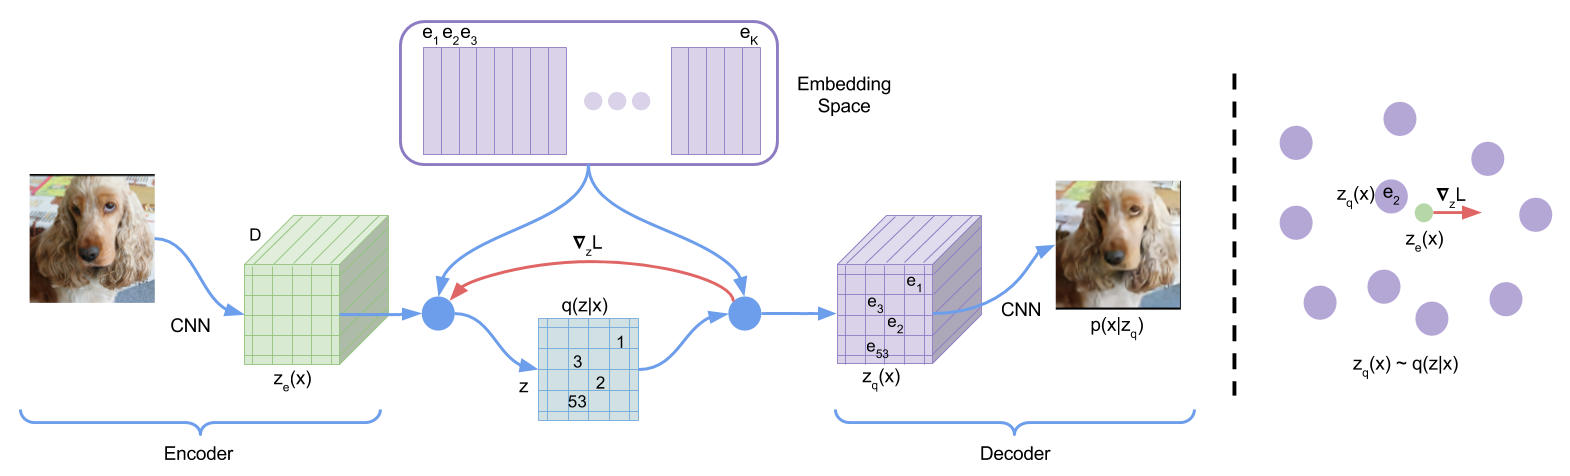
\includegraphics[width=\textwidth]{figures/vq_vae}}
    
    \caption{On the left side there is a figure describing the VQ-VAE architecture. On the right side there is visualization of the latent space whilst training. The figure is taken from~\cite{vqvae}.}
  	\medskip 
	\hspace*{15pt}\hbox{\scriptsize Credit: Aäron van den Oord et al.}\label{VQVAEFigure}
\end{figure}


